\slajdid{04-s002}
\begin{frame}[label=04-s002]{POZICIONI BROJNI SISTEMI}
\gusttekst
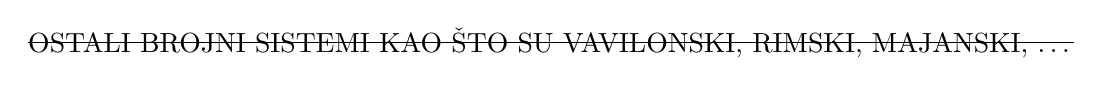
\begin{tikzpicture}
\node[inner sep=0pt,outer sep=0pt] (t) {OSTALI BROJNI SISTEMI KAO ŠTO SU VAVILONSKI, RIMSKI, MAJANSKI, \ldots};
\draw (t.west)--(t.east);
\end{tikzpicture}\par
Hindu-Arabik ili Indo-Arabik\\
Razvoj od 1. do 10. veka nove ere\\
Aryabhata - definisao pozicioni sistem\\
Brahmagupta - uveo nulu\\
Abu'l-Hasan al-Uqlidisi – uveo decimalnu tačku

$r$ – radiks (radix) – osnova brojnog sistema – za nas od interesa kada je to \alert{celobrojna} vrednost

$c_i$ – cifre brojnog sistema\hfill $c_i\in\{0,1,2,\ldots r-2,r-1\}$

$V$ – vrednost koja se prikazuje (za sada samo pozitivne)
\begin{columns}[c,onlytextwidth]
\column{.72\textwidth}
zapis\quad $c_{n-1}c_{n-2}c_{n-3}\ldots c_1\,c_0.\,c_{-1}\,c_{-2}c_{-3}\ldots c_{-k+1}\,c_{-k}$
\[V=\sum_{i=-k}^{n-1}c_i r^i\]
\column{.25\textwidth}
$n$ celih mesta\\$k$ razlomljenih mesta\\. tačka osnove
\end{columns}
Težinski – svaka cifra $c_i$ sa svojom pozicijom $i$ nosi težinu $r^i$
\end{frame}
